\subsection{Distributed SGF FW Experiments}
To test the performance of Algorithm \ref{distributed} we used a distributed network of 10 worker nodes and we
gave them 10 images per class each, for a total of 100 different images each.

Our network is modeled as an undirected simple connected graph $G = (V,E)$, with $V = [1,...,10]$ and $E$ denoting
the connections between nodes. The connectivity of the graph can be computed in the following way: $\Vert W- J \Vert$,
where $J= 11^T/10$ and $11^T$ represents a matrix with all entries set to 1. For the experiment, we have created a network
with a connectivity value of 0.438. The network's connections are determined by the scheme described by the adjacecy
matrix $A$:
\[ A =
\begin{pmatrix}
1& 1& 0& 1& 1& 1& 1& 1& 0& 1\\
1& 1& 1& 0& 1& 1& 1& 0& 1& 1\\
0& 1& 1& 1& 1& 1& 0& 1& 1& 1\\
1& 0& 1& 1& 1& 1& 0& 1& 1& 1\\
1& 1& 1& 1& 1& 1& 1& 0& 1& 1\\
1& 1& 1& 1& 1& 1& 1& 1& 1& 0\\
1& 1& 0& 0& 1& 1& 1& 1& 1& 1\\
1& 0& 1& 1& 0& 1& 1& 1& 1& 1\\
0& 1& 1& 1& 1& 1& 1& 1& 1& 1\\
1& 1& 1& 1& 1& 0& 1& 1& 1& 1
\end{pmatrix}
.\]
Since each node is connected to itself, the diagonal of the matrix A is made of ones.
 Furthermore, we computed the approximated gradient along 15 directions and we tested
the algorithm for 20, 50 and 100 queries.

\begin{figure}%[htbp]
	\centering
	\begin{subfigure}[b]{0.15\textwidth}
		\centering
		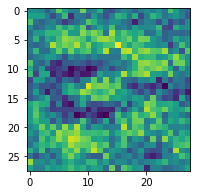
\includegraphics[width=2.5cm]{T20_final_distr.png}
		\caption{}
		\label{fig:distributed_perturbation_20}
	\end{subfigure}
	\hfill
	\begin{subfigure}[b]{0.15\textwidth}
		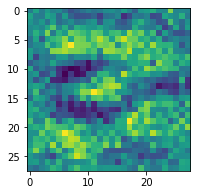
\includegraphics[width=2.5cm]{T50_final_distr.png}
		\caption{}
		\label{fig:variance-distributed_perturbation_50}
	\end{subfigure}
	\hfill
	\begin{subfigure}[b]{0.15\textwidth}
		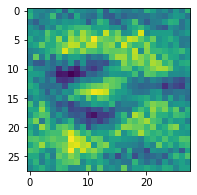
\includegraphics[width=2.5cm]{T100_final_distr.png}
		\caption{}
		\label{fig:distributed_perturbation_100}
	\end{subfigure}
	\caption{Perturbations of the Distributed SGF FW algorithm created for different values of T:
	  \ref{fig:distributed_perturbation_20} for T=20, \ref{fig:variance-distributed_perturbation_50} for T=50, \ref{fig:distributed_perturbation_100} for T=100.}
	\label{fig:perturbations}
\end{figure}

In Figure \ref{fig:perturbations} we can see the universal adversarial perturbations produced by Algorithm \ref{distributed}
for different values of T. As we can clearly see, the three perturbations are very similar to each other and all of
them have a 3 shape.

\begin{figure}[htbp]
	\centering
	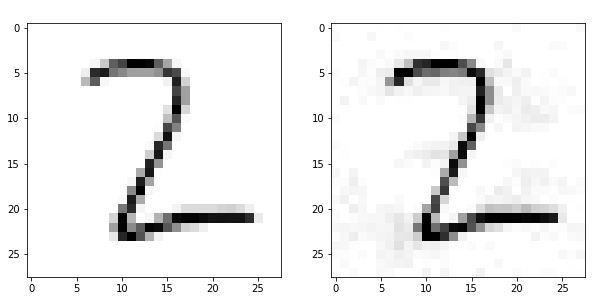
\includegraphics[width=7cm]{image_pertub_T100_final_distr.png}
	\caption{Image of 2 gets classified as 3 after applying the adversarial perturbation generated by the Distributed
	Algorithm \ref{distributed} with 100 queries.}
	\label{fig:distributed}
\end{figure}

In Figure \ref{fig:distributed}, we can see an example of the perturbation created by Algorithm \ref{distributed},
applied to an image of the MNIST digits. As we can see, although we can still recognize the number 3 pattern in the
perturbation, it is much smoother compared to the one we can observe from the perturbation computed by the Decentralized
SGF FW algorithm. Nevertheless, it is strong enough to fool the classifier and lead it to a wrong prediction.

\begin{table}[htbp]
	\begin{center}
		\begin{adjustwidth}{-.6cm}{}
			\begin{tabular}{cccc}
				\textbf{Attack} &          20 \textbf{queries} &      50 \textbf{queries} &     100 \textbf{queries} \\
				\midrule
				{\small Distributed SGF FW}     &   73.47\% &    74.62\% &       75.84\% \\
			\end{tabular}
		\end{adjustwidth}
	\end{center}
	\caption{{\small Summary of $\ell_\infty$ Universal Adversarial Perturbation with $\varepsilon$=0.25. MNIST attack using Distributed
	SGF FW. The number of queries denotes the number of queries used per image.}}
	\label{tab:distributed}
\end{table}

In Table \ref{tab:distributed} are displayed the values of accuracy reached by the LeNet-5 classifier on perturbed images.